\documentclass[11pt]{article}
\renewcommand{\arraystretch}{1.5} % Default value: 1
\usepackage{sectsty}
\allsectionsfont{\color{blue}\fontfamily{lmss}\selectfont}
\usepackage{fontspec}
\setmainfont{XCharter}

\usepackage{listings}
\lstset{
basicstyle=\small\ttfamily,
tabsize=8,
columns=flexible,
breaklines=true,
frame=tb,
rulecolor=\color[rgb]{0.8,0.8,0.7},
backgroundcolor=\color[rgb]{1,1,0.91},
postbreak=\raisebox{0ex}[0ex][0ex]{\ensuremath{\color{red}\hookrightarrow\space}}
}
\usepackage{fontawesome}


\usepackage{mdframed}
\newmdenv[
  backgroundcolor=gray,
  fontcolor=white,
  nobreak=true,
]{terminalinput}



\usepackage{parskip}




    \usepackage[T1]{fontenc}
    % Nicer default font (+ math font) than Computer Modern for most use cases
    \usepackage{mathpazo}

    % Basic figure setup, for now with no caption control since it's done
    % automatically by Pandoc (which extracts ![](path) syntax from Markdown).
    \usepackage{graphicx}
    % We will generate all images so they have a width \maxwidth. This means
    % that they will get their normal width if they fit onto the page, but
    % are scaled down if they would overflow the margins.
    \makeatletter
    \def\maxwidth{\ifdim\Gin@nat@width>\linewidth\linewidth
    \else\Gin@nat@width\fi}
    \makeatother
    \let\Oldincludegraphics\includegraphics
    % Set max figure width to be 80% of text width, for now hardcoded.
\renewcommand{\includegraphics}[1]{\Oldincludegraphics[width=.8\maxwidth, height=.55\textheight, keepaspectratio]{#1}}
    % Ensure that by default, figures have no caption (until we provide a
    % proper Figure object with a Caption API and a way to capture that
    % in the conversion process - todo).
    \usepackage{caption}
    \DeclareCaptionLabelFormat{nolabel}{}
    \captionsetup{labelformat=nolabel, textfont=bf}

    \usepackage{adjustbox} % Used to constrain images to a maximum size
    \usepackage{xcolor} % Allow colors to be defined
    \usepackage{enumerate} % Needed for markdown enumerations to work
    \usepackage{geometry} % Used to adjust the document margins
    \usepackage{amsmath} % Equations
    \usepackage{amssymb} % Equations
    \usepackage{textcomp} % defines textquotesingle
    % Hack from http://tex.stackexchange.com/a/47451/13684:
    \AtBeginDocument{%
        \def\PYZsq{\textquotesingle}% Upright quotes in Pygmentized code
    }
    \usepackage{upquote} % Upright quotes for verbatim code
    \usepackage{eurosym} % defines \euro
    \usepackage[mathletters]{ucs} % Extended unicode (utf-8) support
    \usepackage[utf8x]{inputenc} % Allow utf-8 characters in the tex document
    \usepackage{fancyvrb} % verbatim replacement that allows latex
    \usepackage{grffile} % extends the file name processing of package graphics
                         % to support a larger range
    % The hyperref package gives us a pdf with properly built
    % internal navigation ('pdf bookmarks' for the table of contents,
    % internal cross-reference links, web links for URLs, etc.)
    \usepackage{hyperref}
    \usepackage{longtable} % longtable support required by pandoc >1.10
    \usepackage{booktabs}  % table support for pandoc > 1.12.2
    \usepackage[inline]{enumitem} % IRkernel/repr support (it uses the enumerate* environment)
    \usepackage[normalem]{ulem} % ulem is needed to support strikethroughs (\sout)
                                % normalem makes italics be italics, not underlines




    % Colors for the hyperref package
    \definecolor{urlcolor}{rgb}{0,.145,.698}
    \definecolor{linkcolor}{rgb}{.71,0.21,0.01}
    \definecolor{citecolor}{rgb}{.12,.54,.11}

    % ANSI colors
    \definecolor{ansi-black}{HTML}{3E424D}
    \definecolor{ansi-black-intense}{HTML}{282C36}
    \definecolor{ansi-red}{HTML}{E75C58}
    \definecolor{ansi-red-intense}{HTML}{B22B31}
    \definecolor{ansi-green}{HTML}{00A250}
    \definecolor{ansi-green-intense}{HTML}{007427}
    \definecolor{ansi-yellow}{HTML}{DDB62B}
    \definecolor{ansi-yellow-intense}{HTML}{B27D12}
    \definecolor{ansi-blue}{HTML}{208FFB}
    \definecolor{ansi-blue-intense}{HTML}{0065CA}
    \definecolor{ansi-magenta}{HTML}{D160C4}
    \definecolor{ansi-magenta-intense}{HTML}{A03196}
    \definecolor{ansi-cyan}{HTML}{60C6C8}
    \definecolor{ansi-cyan-intense}{HTML}{258F8F}
    \definecolor{ansi-white}{HTML}{C5C1B4}
    \definecolor{ansi-white-intense}{HTML}{A1A6B2}

    % commands and environments needed by pandoc snippets
    % extracted from the output of `pandoc -s`
    \providecommand{\tightlist}{%
      \setlength{\itemsep}{0pt}\setlength{\parskip}{0pt}}
    \DefineVerbatimEnvironment{Highlighting}{Verbatim}{commandchars=\\\{\}}
    % Add ',fontsize=\small' for more characters per line
    \newenvironment{Shaded}{}{}
    \newcommand{\KeywordTok}[1]{\textcolor[rgb]{0.00,0.44,0.13}{\textbf{{#1}}}}
    \newcommand{\DataTypeTok}[1]{\textcolor[rgb]{0.56,0.13,0.00}{{#1}}}
    \newcommand{\DecValTok}[1]{\textcolor[rgb]{0.25,0.63,0.44}{{#1}}}
    \newcommand{\BaseNTok}[1]{\textcolor[rgb]{0.25,0.63,0.44}{{#1}}}
    \newcommand{\FloatTok}[1]{\textcolor[rgb]{0.25,0.63,0.44}{{#1}}}
    \newcommand{\CharTok}[1]{\textcolor[rgb]{0.25,0.44,0.63}{{#1}}}
    \newcommand{\StringTok}[1]{\textcolor[rgb]{0.25,0.44,0.63}{{#1}}}
    \newcommand{\CommentTok}[1]{\textcolor[rgb]{0.38,0.63,0.69}{\textit{{#1}}}}
    \newcommand{\OtherTok}[1]{\textcolor[rgb]{0.00,0.44,0.13}{{#1}}}
    \newcommand{\AlertTok}[1]{\textcolor[rgb]{1.00,0.00,0.00}{\textbf{{#1}}}}
    \newcommand{\FunctionTok}[1]{\textcolor[rgb]{0.02,0.16,0.49}{{#1}}}
    \newcommand{\RegionMarkerTok}[1]{{#1}}
    \newcommand{\ErrorTok}[1]{\textcolor[rgb]{1.00,0.00,0.00}{\textbf{{#1}}}}
    \newcommand{\NormalTok}[1]{{#1}}

    % Additional commands for more recent versions of Pandoc
    \newcommand{\ConstantTok}[1]{\textcolor[rgb]{0.53,0.00,0.00}{{#1}}}
    \newcommand{\SpecialCharTok}[1]{\textcolor[rgb]{0.25,0.44,0.63}{{#1}}}
    \newcommand{\VerbatimStringTok}[1]{\textcolor[rgb]{0.25,0.44,0.63}{{#1}}}
    \newcommand{\SpecialStringTok}[1]{\textcolor[rgb]{0.73,0.40,0.53}{{#1}}}
    \newcommand{\ImportTok}[1]{{#1}}
    \newcommand{\DocumentationTok}[1]{\textcolor[rgb]{0.73,0.13,0.13}{\textit{{#1}}}}
    \newcommand{\AnnotationTok}[1]{\textcolor[rgb]{0.38,0.63,0.69}{\textbf{\textit{{#1}}}}}
    \newcommand{\CommentVarTok}[1]{\textcolor[rgb]{0.38,0.63,0.69}{\textbf{\textit{{#1}}}}}
    \newcommand{\VariableTok}[1]{\textcolor[rgb]{0.10,0.09,0.49}{{#1}}}
    \newcommand{\ControlFlowTok}[1]{\textcolor[rgb]{0.00,0.44,0.13}{\textbf{{#1}}}}
    \newcommand{\OperatorTok}[1]{\textcolor[rgb]{0.40,0.40,0.40}{{#1}}}
    \newcommand{\BuiltInTok}[1]{{#1}}
    \newcommand{\ExtensionTok}[1]{{#1}}
    \newcommand{\PreprocessorTok}[1]{\textcolor[rgb]{0.74,0.48,0.00}{{#1}}}
    \newcommand{\AttributeTok}[1]{\textcolor[rgb]{0.49,0.56,0.16}{{#1}}}
    \newcommand{\InformationTok}[1]{\textcolor[rgb]{0.38,0.63,0.69}{\textbf{\textit{{#1}}}}}
    \newcommand{\WarningTok}[1]{\textcolor[rgb]{0.38,0.63,0.69}{\textbf{\textit{{#1}}}}}


    % Define a nice break command that doesn't care if a line doesn't already
    % exist.
    \def\br{\hspace*{\fill} \\* }
    % Math Jax compatability definitions
    \def\gt{>}
    \def\lt{<}
    % Document parameters
    \title{ChIPSeq-Project1}




    % Pygments definitions

\makeatletter
\def\PY@reset{\let\PY@it=\relax \let\PY@bf=\relax%
    \let\PY@ul=\relax \let\PY@tc=\relax%
    \let\PY@bc=\relax \let\PY@ff=\relax}
\def\PY@tok#1{\csname PY@tok@#1\endcsname}
\def\PY@toks#1+{\ifx\relax#1\empty\else%
    \PY@tok{#1}\expandafter\PY@toks\fi}
\def\PY@do#1{\PY@bc{\PY@tc{\PY@ul{%
    \PY@it{\PY@bf{\PY@ff{#1}}}}}}}
\def\PY#1#2{\PY@reset\PY@toks#1+\relax+\PY@do{#2}}

\expandafter\def\csname PY@tok@kr\endcsname{\let\PY@bf=\textbf\def\PY@tc##1{\textcolor[rgb]{0.00,0.50,0.00}{##1}}}
\expandafter\def\csname PY@tok@gs\endcsname{\let\PY@bf=\textbf}
\expandafter\def\csname PY@tok@sx\endcsname{\def\PY@tc##1{\textcolor[rgb]{0.00,0.50,0.00}{##1}}}
\expandafter\def\csname PY@tok@ge\endcsname{\let\PY@it=\textit}
\expandafter\def\csname PY@tok@no\endcsname{\def\PY@tc##1{\textcolor[rgb]{0.53,0.00,0.00}{##1}}}
\expandafter\def\csname PY@tok@sb\endcsname{\def\PY@tc##1{\textcolor[rgb]{0.73,0.13,0.13}{##1}}}
\expandafter\def\csname PY@tok@nn\endcsname{\let\PY@bf=\textbf\def\PY@tc##1{\textcolor[rgb]{0.00,0.00,1.00}{##1}}}
\expandafter\def\csname PY@tok@gp\endcsname{\let\PY@bf=\textbf\def\PY@tc##1{\textcolor[rgb]{0.00,0.00,0.50}{##1}}}
\expandafter\def\csname PY@tok@nd\endcsname{\def\PY@tc##1{\textcolor[rgb]{0.67,0.13,1.00}{##1}}}
\expandafter\def\csname PY@tok@c\endcsname{\let\PY@it=\textit\def\PY@tc##1{\textcolor[rgb]{0.25,0.50,0.50}{##1}}}
\expandafter\def\csname PY@tok@ne\endcsname{\let\PY@bf=\textbf\def\PY@tc##1{\textcolor[rgb]{0.82,0.25,0.23}{##1}}}
\expandafter\def\csname PY@tok@cm\endcsname{\let\PY@it=\textit\def\PY@tc##1{\textcolor[rgb]{0.25,0.50,0.50}{##1}}}
\expandafter\def\csname PY@tok@kd\endcsname{\let\PY@bf=\textbf\def\PY@tc##1{\textcolor[rgb]{0.00,0.50,0.00}{##1}}}
\expandafter\def\csname PY@tok@sh\endcsname{\def\PY@tc##1{\textcolor[rgb]{0.73,0.13,0.13}{##1}}}
\expandafter\def\csname PY@tok@s2\endcsname{\def\PY@tc##1{\textcolor[rgb]{0.73,0.13,0.13}{##1}}}
\expandafter\def\csname PY@tok@cpf\endcsname{\let\PY@it=\textit\def\PY@tc##1{\textcolor[rgb]{0.25,0.50,0.50}{##1}}}
\expandafter\def\csname PY@tok@s1\endcsname{\def\PY@tc##1{\textcolor[rgb]{0.73,0.13,0.13}{##1}}}
\expandafter\def\csname PY@tok@nt\endcsname{\let\PY@bf=\textbf\def\PY@tc##1{\textcolor[rgb]{0.00,0.50,0.00}{##1}}}
\expandafter\def\csname PY@tok@kp\endcsname{\def\PY@tc##1{\textcolor[rgb]{0.00,0.50,0.00}{##1}}}
\expandafter\def\csname PY@tok@cs\endcsname{\let\PY@it=\textit\def\PY@tc##1{\textcolor[rgb]{0.25,0.50,0.50}{##1}}}
\expandafter\def\csname PY@tok@si\endcsname{\let\PY@bf=\textbf\def\PY@tc##1{\textcolor[rgb]{0.73,0.40,0.53}{##1}}}
\expandafter\def\csname PY@tok@m\endcsname{\def\PY@tc##1{\textcolor[rgb]{0.40,0.40,0.40}{##1}}}
\expandafter\def\csname PY@tok@ow\endcsname{\let\PY@bf=\textbf\def\PY@tc##1{\textcolor[rgb]{0.67,0.13,1.00}{##1}}}
\expandafter\def\csname PY@tok@nl\endcsname{\def\PY@tc##1{\textcolor[rgb]{0.63,0.63,0.00}{##1}}}
\expandafter\def\csname PY@tok@kc\endcsname{\let\PY@bf=\textbf\def\PY@tc##1{\textcolor[rgb]{0.00,0.50,0.00}{##1}}}
\expandafter\def\csname PY@tok@se\endcsname{\let\PY@bf=\textbf\def\PY@tc##1{\textcolor[rgb]{0.73,0.40,0.13}{##1}}}
\expandafter\def\csname PY@tok@sc\endcsname{\def\PY@tc##1{\textcolor[rgb]{0.73,0.13,0.13}{##1}}}
\expandafter\def\csname PY@tok@nc\endcsname{\let\PY@bf=\textbf\def\PY@tc##1{\textcolor[rgb]{0.00,0.00,1.00}{##1}}}
\expandafter\def\csname PY@tok@kt\endcsname{\def\PY@tc##1{\textcolor[rgb]{0.69,0.00,0.25}{##1}}}
\expandafter\def\csname PY@tok@mi\endcsname{\def\PY@tc##1{\textcolor[rgb]{0.40,0.40,0.40}{##1}}}
\expandafter\def\csname PY@tok@vc\endcsname{\def\PY@tc##1{\textcolor[rgb]{0.10,0.09,0.49}{##1}}}
\expandafter\def\csname PY@tok@w\endcsname{\def\PY@tc##1{\textcolor[rgb]{0.73,0.73,0.73}{##1}}}
\expandafter\def\csname PY@tok@na\endcsname{\def\PY@tc##1{\textcolor[rgb]{0.49,0.56,0.16}{##1}}}
\expandafter\def\csname PY@tok@mb\endcsname{\def\PY@tc##1{\textcolor[rgb]{0.40,0.40,0.40}{##1}}}
\expandafter\def\csname PY@tok@mh\endcsname{\def\PY@tc##1{\textcolor[rgb]{0.40,0.40,0.40}{##1}}}
\expandafter\def\csname PY@tok@gd\endcsname{\def\PY@tc##1{\textcolor[rgb]{0.63,0.00,0.00}{##1}}}
\expandafter\def\csname PY@tok@il\endcsname{\def\PY@tc##1{\textcolor[rgb]{0.40,0.40,0.40}{##1}}}
\expandafter\def\csname PY@tok@ch\endcsname{\let\PY@it=\textit\def\PY@tc##1{\textcolor[rgb]{0.25,0.50,0.50}{##1}}}
\expandafter\def\csname PY@tok@vi\endcsname{\def\PY@tc##1{\textcolor[rgb]{0.10,0.09,0.49}{##1}}}
\expandafter\def\csname PY@tok@gr\endcsname{\def\PY@tc##1{\textcolor[rgb]{1.00,0.00,0.00}{##1}}}
\expandafter\def\csname PY@tok@vg\endcsname{\def\PY@tc##1{\textcolor[rgb]{0.10,0.09,0.49}{##1}}}
\expandafter\def\csname PY@tok@nf\endcsname{\def\PY@tc##1{\textcolor[rgb]{0.00,0.00,1.00}{##1}}}
\expandafter\def\csname PY@tok@err\endcsname{\def\PY@bc##1{\setlength{\fboxsep}{0pt}\fcolorbox[rgb]{1.00,0.00,0.00}{1,1,1}{\strut ##1}}}
\expandafter\def\csname PY@tok@mo\endcsname{\def\PY@tc##1{\textcolor[rgb]{0.40,0.40,0.40}{##1}}}
\expandafter\def\csname PY@tok@o\endcsname{\def\PY@tc##1{\textcolor[rgb]{0.40,0.40,0.40}{##1}}}
\expandafter\def\csname PY@tok@gt\endcsname{\def\PY@tc##1{\textcolor[rgb]{0.00,0.27,0.87}{##1}}}
\expandafter\def\csname PY@tok@s\endcsname{\def\PY@tc##1{\textcolor[rgb]{0.73,0.13,0.13}{##1}}}
\expandafter\def\csname PY@tok@sd\endcsname{\let\PY@it=\textit\def\PY@tc##1{\textcolor[rgb]{0.73,0.13,0.13}{##1}}}
\expandafter\def\csname PY@tok@c1\endcsname{\let\PY@it=\textit\def\PY@tc##1{\textcolor[rgb]{0.25,0.50,0.50}{##1}}}
\expandafter\def\csname PY@tok@k\endcsname{\let\PY@bf=\textbf\def\PY@tc##1{\textcolor[rgb]{0.00,0.50,0.00}{##1}}}
\expandafter\def\csname PY@tok@mf\endcsname{\def\PY@tc##1{\textcolor[rgb]{0.40,0.40,0.40}{##1}}}
\expandafter\def\csname PY@tok@gh\endcsname{\let\PY@bf=\textbf\def\PY@tc##1{\textcolor[rgb]{0.00,0.00,0.50}{##1}}}
\expandafter\def\csname PY@tok@ni\endcsname{\let\PY@bf=\textbf\def\PY@tc##1{\textcolor[rgb]{0.60,0.60,0.60}{##1}}}
\expandafter\def\csname PY@tok@kn\endcsname{\let\PY@bf=\textbf\def\PY@tc##1{\textcolor[rgb]{0.00,0.50,0.00}{##1}}}
\expandafter\def\csname PY@tok@go\endcsname{\def\PY@tc##1{\textcolor[rgb]{0.53,0.53,0.53}{##1}}}
\expandafter\def\csname PY@tok@nv\endcsname{\def\PY@tc##1{\textcolor[rgb]{0.10,0.09,0.49}{##1}}}
\expandafter\def\csname PY@tok@gu\endcsname{\let\PY@bf=\textbf\def\PY@tc##1{\textcolor[rgb]{0.50,0.00,0.50}{##1}}}
\expandafter\def\csname PY@tok@sr\endcsname{\def\PY@tc##1{\textcolor[rgb]{0.73,0.40,0.53}{##1}}}
\expandafter\def\csname PY@tok@cp\endcsname{\def\PY@tc##1{\textcolor[rgb]{0.74,0.48,0.00}{##1}}}
\expandafter\def\csname PY@tok@bp\endcsname{\def\PY@tc##1{\textcolor[rgb]{0.00,0.50,0.00}{##1}}}
\expandafter\def\csname PY@tok@ss\endcsname{\def\PY@tc##1{\textcolor[rgb]{0.10,0.09,0.49}{##1}}}
\expandafter\def\csname PY@tok@gi\endcsname{\def\PY@tc##1{\textcolor[rgb]{0.00,0.63,0.00}{##1}}}
\expandafter\def\csname PY@tok@nb\endcsname{\def\PY@tc##1{\textcolor[rgb]{0.00,0.50,0.00}{##1}}}

\def\PYZbs{\char`\\}
\def\PYZus{\char`\_}
\def\PYZob{\char`\{}
\def\PYZcb{\char`\}}
\def\PYZca{\char`\^}
\def\PYZam{\char`\&}
\def\PYZlt{\char`\<}
\def\PYZgt{\char`\>}
\def\PYZsh{\char`\#}
\def\PYZpc{\char`\%}
\def\PYZdl{\char`\$}
\def\PYZhy{\char`\-}
\def\PYZsq{\char`\'}
\def\PYZdq{\char`\"}
\def\PYZti{\char`\~}
% for compatibility with earlier versions
\def\PYZat{@}
\def\PYZlb{[}
\def\PYZrb{]}
\makeatother


    % Exact colors from NB
    \definecolor{incolor}{rgb}{0.0, 0.0, 0.5}
    \definecolor{outcolor}{rgb}{0.545, 0.0, 0.0}




    % Prevent overflowing lines due to hard-to-break entities
    \sloppy
    % Setup hyperref package
    \hypersetup{
      breaklinks=true,  % so long urls are correctly broken across lines
      colorlinks=true,
      urlcolor=urlcolor,
      linkcolor=linkcolor,
      citecolor=citecolor,
      }
    % Slightly bigger margins than the latex defaults

    \geometry{verbose,tmargin=1in,bmargin=1in,lmargin=1in,rmargin=1in}



\renewcommand{\PY}[2]{{#2}}
\usepackage{fancyhdr}
\pagestyle{fancy}
\rhead{\color{gray}\sf\small\rightmark}
\lhead{\nouppercase{\color{gray}\sf\small\leftmark}}
\cfoot{\color{gray}\sf\thepage}
\renewcommand{\footrulewidth}{1pt}
\begin{document}






    \section{ChIP-Seq Project 1: Sequencing depth and Chromatin
Environment}\label{chip-seq-project-1-sequencing-depth-and-chromatin-environment}

    The following tasks have been adapted from materials developed by Angela
Goncalves, Myrto Kostadima, Steven Wilder and Maria Xenophontos.

    \subsection{Sequencing depth}\label{sequencing-depth}

    One of the most frequent questions that come up in ChIP-seq experiments
is whether the sequencing depth is sufficient.

The more we sequence a ChIP-seq library, the more peaks of low fold
change we will identify. Therefore, the only way to answer that question
is to look for the number of peaks identified when we down sample our
library. To test for sufficient sequencing depth in our sample we will
down sample our ChIP and Control datasets to 10\%, 20\%, .., 90\% of the
initial library size and call peaks. To do so, we will use the functions
\textbf{randsample} and \textbf{callpeak} from macs2, respectively.

\textbf{First, go to the group\_projects folder.}

\begin{terminalinput}
\begin{Verbatim}[commandchars=\\\{\}]
\llap{\color{black}\LARGE\faKeyboardO\hspace{1em}} \PY{n+nb}{cd} /home/manager/course\PYZus{}data/group\PYZus{}projects
\end{Verbatim}
\end{terminalinput}


    \textbf{Check to see if the ChIPSeq-Project1 folder exists.}

\begin{terminalinput}
\begin{Verbatim}[commandchars=\\\{\}]
\llap{\color{black}\LARGE\faKeyboardO\hspace{1em}} ls ChIPSeq\PYZhy{}Project1
\end{Verbatim}
\end{terminalinput}


    \textbf{If this folder doesn't exist, please check with your course
instructor.}

    \textbf{Once you have the data, go into the ChIPSeq-Project1 directory.}

\begin{terminalinput}
\begin{Verbatim}[commandchars=\\\{\}]
\llap{\color{black}\LARGE\faKeyboardO\hspace{1em}} \PY{n+nb}{cd} ChIPSeq\PYZhy{}Project1
\end{Verbatim}
\end{terminalinput}


    Below are a series of commands which will downsample the ChIP and
Control datasets to 10\%, 20\%, .., 90\% of the initial library size and
call peaks. To do this we use a while loop which will start counting
from 10 (\texttt{i=10}), in intervals of 10 (e.g. 10, 20, 30...)
(\texttt{((i\ =\ i\ +\ 10))}) up to 100 (\texttt{\$i\ -lt\ 100}). The
value which is being counted is stored in a variable called \texttt{i}
that is then referenced in other commands using \texttt{\$i}. Finally,
to make sure we know where we are in the loop, we will print a message
in the terminal \texttt{echo\ "Looking\ at\ \$\{i\}\%\ of\ the\ reads"}.

The command we are using to downsample the ChIP and Control datasets
reads is \texttt{macs2\ randsample} which we will be giving an input
file \texttt{-t}, a percentage \texttt{-p}, an output file \texttt{-o},
an output directory \texttt{-\/-outdir} and the format of the input file
\texttt{-f}.

\textbf{Look at the usage for \texttt{macs2\ randsample}.}

\begin{terminalinput}
\begin{Verbatim}[commandchars=\\\{\}]
\llap{\color{black}\LARGE\faKeyboardO\hspace{1em}} macs2 randsample \PYZhy{}h
\end{Verbatim}
\end{terminalinput}


    We then call the peaks for each set of downsampled reads using
\texttt{macs2\ callpeak} in a similar way to the ChIP-Seq tutorial.

\newpage

\textbf{Type the commands below into a file called
\texttt{project1.sh}.}

\begin{terminalinput}
\begin{Verbatim}[commandchars=\\\{\}]
\llap{\color{black}\LARGE\faKeyboardO\hspace{1em}} \PY{n+nv}{i}\PY{o}{=}10

        \PY{k}{while} \PY{o}{[}\PY{o}{[} \PY{n+nv}{\PYZdl{}i} \PYZhy{}lt \PY{l+m}{100} \PY{o}{]}\PY{o}{]}
        \PY{k}{do}

        \PY{n+nb}{echo} \PY{l+s+s2}{\PYZdq{}}\PY{l+s+s2}{Looking at }\PY{l+s+si}{\PYZdl{}\PYZob{}}\PY{n+nv}{i}\PY{l+s+si}{\PYZcb{}}\PY{l+s+s2}{\PYZpc{} of the reads}\PY{l+s+s2}{\PYZdq{}}

        macs2 randsample \PYZhy{}t PAX5.bam \PYZhy{}p \PY{n+nv}{\PYZdl{}i} \PYZhy{}o PAX5.perc\PY{l+s+si}{\PYZdl{}\PYZob{}}\PY{n+nv}{i}\PY{l+s+si}{\PYZcb{}}.bed \PY{l+s+se}{\PYZbs{}}
        \PYZhy{}\PYZhy{}outdir macs2\PYZus{}downsample \PYZhy{}f BAM

        macs2 randsample \PYZhy{}t Control.bam \PYZhy{}p \PY{n+nv}{\PYZdl{}i} \PYZhy{}o Control.perc\PY{l+s+si}{\PYZdl{}\PYZob{}}\PY{n+nv}{i}\PY{l+s+si}{\PYZcb{}}.bed \PY{l+s+se}{\PYZbs{}}
        \PYZhy{}\PYZhy{}outdir macs2\PYZus{}downsample \PYZhy{}f BAM

        macs2 callpeak \PYZhy{}t macs2\PYZus{}downsample/PAX5.perc\PY{l+s+si}{\PYZdl{}\PYZob{}}\PY{n+nv}{i}\PY{l+s+si}{\PYZcb{}}.bed \PY{l+s+se}{\PYZbs{}}
        \PYZhy{}c macs2\PYZus{}downsample/Control.perc\PY{l+s+si}{\PYZdl{}\PYZob{}}\PY{n+nv}{i}\PY{l+s+si}{\PYZcb{}}.bed \PYZhy{}\PYZhy{}gsize \PY{l+m}{138000000} \PY{l+s+se}{\PYZbs{}}
        \PYZhy{}\PYZhy{}format BED \PYZhy{}\PYZhy{}name macs2\PYZus{}downsample/PAX5.perc\PY{l+s+si}{\PYZdl{}\PYZob{}}\PY{n+nv}{i}\PY{l+s+si}{\PYZcb{}} \PY{l+s+se}{\PYZbs{}}
        \PYZhy{}\PYZhy{}pvalue 1e\PYZhy{}3 \PYZhy{}\PYZhy{}call\PYZhy{}summits

        \PY{o}{(}\PY{o}{(}\PY{n+nv}{i} \PY{o}{=} i + 10\PY{o}{)}\PY{o}{)}

        \PY{k}{done}
\end{Verbatim}
\end{terminalinput}


    \textbf{Now, make your script executable.}

\begin{terminalinput}
\begin{Verbatim}[commandchars=\\\{\}]
\llap{\color{black}\LARGE\faKeyboardO\hspace{1em}} chmod u+x project1.sh
\end{Verbatim}
\end{terminalinput}


    \textbf{And run the script.}

\begin{terminalinput}
\begin{Verbatim}[commandchars=\\\{\}]
\llap{\color{black}\LARGE\faKeyboardO\hspace{1em}} ./project1.sh
\end{Verbatim}
\end{terminalinput}


    Next, we want to plot the number of peaks called in each of the
downsampled datasets. To do this we will use \texttt{R}. First we tell R
where to find our output files using \texttt{setwd}. We then use a for
loop to extract only the peaks whose overall enrichment meets a
threshold value (\texttt{fc.thres\ \textless{}-\ 4} and
\texttt{peaks\ \textless{}-\ peaks{[}peaks{[},\ 7{]}\ \textgreater{}\ fc.thres,\ {]}}).
We then count those peaks
(\texttt{no.peaks\ \textless{}-\ c(no.peaks,\ nrow(peaks))}). Finally,
we plot the number of peaks vs the percentage, saving the output to
\texttt{peaks\_vs\_percentage.jpg}.

\newpage

    \textbf{Type the following commands into a file called
\texttt{script.R}.}

\begin{terminalinput}
\begin{Verbatim}[commandchars=\\\{\}]
\llap{\color{black}\LARGE\faKeyboardO\hspace{1em}} rm\PY{o}{(}\PY{n+nv}{list} \PY{o}{=} ls\PY{o}{(}\PY{o}{)}\PY{o}{)}

        options\PY{o}{(}\PY{n+nv}{stringsAsFactors}\PY{o}{=}F\PY{o}{)}
        setwd\PY{o}{(} \PY{l+s+s2}{\PYZdq{}/home/manager/course\PYZus{}data/group\PYZus{}projects/ChIPSeq\PYZhy{}Project1\PYZdq{}} \PY{o}{)}

        fc.thres \PYZlt{}\PYZhy{} 4

        no.peaks \PYZlt{}\PYZhy{} c\PY{o}{(}\PY{o}{)}
        \PY{k}{for}\PY{o}{(}row in seq\PY{o}{(}\PY{n+nv}{from}\PY{o}{=}10, \PY{n+nv}{to} \PY{o}{=} 90, \PY{n+nv}{by} \PY{o}{=} 10\PY{o}{)}\PY{o}{)}
        \PY{o}{\PYZob{}}
        	print\PY{o}{(}row\PY{o}{)}

        	peaks \PYZlt{}\PYZhy{} read.table\PY{o}{(}paste\PY{o}{(}\PY{l+s+s2}{\PYZdq{}macs2\PYZus{}downsample/PAX5.perc\PYZdq{}},
            row, \PY{l+s+s2}{\PYZdq{}\PYZus{}peaks.narrowPeak\PYZdq{}}, \PY{n+nv}{sep}\PY{o}{=}\PY{l+s+s2}{\PYZdq{}\PYZdq{}}\PY{o}{)}\PY{o}{)}

        	peaks \PYZlt{}\PYZhy{} peaks\PY{o}{[}peaks\PY{o}{[}, 7\PY{o}{]} \PYZgt{} fc.thres, \PY{o}{]}

        	no.peaks \PYZlt{}\PYZhy{} c\PY{o}{(}no.peaks, nrow\PY{o}{(}peaks\PY{o}{)}\PY{o}{)}
        \PY{o}{\PYZcb{}}

        peaks \PYZlt{}\PYZhy{} read.table\PY{o}{(}\PY{l+s+s2}{\PYZdq{}PAX5\PYZus{}peaks.narrowPeak\PYZdq{}}\PY{o}{)}
        peaks \PYZlt{}\PYZhy{} peaks\PY{o}{[}peaks\PY{o}{[}, 7\PY{o}{]} \PYZgt{} fc.thres, \PY{o}{]}
        no.peaks \PYZlt{}\PYZhy{} c\PY{o}{(}no.peaks, nrow\PY{o}{(}peaks\PY{o}{)}\PY{o}{)}


        jpeg\PY{o}{(}\PY{l+s+s1}{\PYZsq{}peaks\PYZus{}vs\PYZus{}percentage.jpg\PYZsq{}}\PY{o}{)}

        plot\PY{o}{(}seq\PY{o}{(}\PY{n+nv}{from}\PY{o}{=}10, \PY{n+nv}{to} \PY{o}{=} 100, \PY{n+nv}{by} \PY{o}{=} 10\PY{o}{)}, no.peaks,
        \PY{n+nv}{type}\PY{o}{=}\PY{l+s+s2}{\PYZdq{}o\PYZdq{}}, \PY{n+nv}{col}\PY{o}{=}\PY{l+s+s2}{\PYZdq{}blue\PYZdq{}}, \PY{n+nv}{xlab}\PY{o}{=}\PY{l+s+s2}{\PYZdq{}Percentage of reads\PYZdq{}}, \PY{n+nv}{ylab}\PY{o}{=}\PY{l+s+s2}{\PYZdq{}Number of peaks\PYZdq{}}\PY{o}{)}

        dev.off\PY{o}{(}\PY{o}{)}
\end{Verbatim}
\end{terminalinput}


    \textbf{Use \texttt{Rscript} to run your R script.}

\begin{terminalinput}
\begin{Verbatim}[commandchars=\\\{\}]
\llap{\color{black}\LARGE\faKeyboardO\hspace{1em}} Rscript script.R
\end{Verbatim}
\end{terminalinput}


    \textbf{Let's take a look at the plot.}

\begin{terminalinput}
\begin{Verbatim}[commandchars=\\\{\}]
\llap{\color{black}\LARGE\faKeyboardO\hspace{1em}} eog peaks\PYZus{}vs\PYZus{}percentage.jpg
\end{Verbatim}
\end{terminalinput}


    \textbf{Q1: Do you think that we have sequenced enough?}

    Close the file when you have finished looking at the plot.

\newpage

    \subsection{Chromatin Environment}\label{chromatin-environment}

    The goal of this hands-on session is to investigate the chromatin
environment around gene features and regulatory elements. We will be
plotting where the different histone modifications occur in relation to
genes. We will also look at how we can distinguish different genes based
on transcription and chromatin environment.

    \subsubsection{Prepare environment}\label{prepare-environment}

    We will be using ENCODE GM12878 histone modifications. The BAM alignment
files have been downloaded from http://www.encodeproject.org. All ENCODE
experiments had at least 2 technical replicates, but we will only be
using the first replicate for simplicity.

We will be using \textbf{ngsplot}
https://github.com/shenlab-sinai/ngsplot to visualise these datasets at
transcription start sites. The ngsplot database for the human gene set
has been generated from the Ensembl http://www.ensembl.org and RefSeq
http://www.ncbi.nlm.nih.gov/refseq/ gene sets, by default using the
Ensembl set.

    \textbf{Make sure that the location where we want to write the database
to is writable.}

\begin{terminalinput}
\begin{Verbatim}[commandchars=\\\{\}]
\llap{\color{black}\LARGE\faKeyboardO\hspace{1em}} sudo chmod \PYZhy{}R \PY{l+m}{777} /usr/local/bioinf\PYZhy{}recipes/ngsplot\PYZhy{}2.63
\end{Verbatim}
\end{terminalinput}


    \textbf{When prompted, type the password for manager which is
\texttt{manager}.}

    \textbf{Next, make sure that the following R libraries are installed.}

\begin{terminalinput}
\begin{Verbatim}[commandchars=\\\{\}]
\llap{\color{black}\LARGE\faKeyboardO\hspace{1em}} sudo R
\end{Verbatim}
\end{terminalinput}


    \textbf{In R, type the following commands. When prompted, type
\texttt{n} so that other packages are not updated.}

    \begin{verbatim}
source("https://bioconductor.org/biocLite.R")
BiocInstaller::biocLite(c("ShortRead", "BSgenome", "doMC"))
\end{verbatim}

    \textbf{To quit R type \texttt{q()} and enter \texttt{n} when prompted.}

    \textbf{Now, install the database using \texttt{ngsplotdb.py}.}

\begin{terminalinput}
\begin{Verbatim}[commandchars=\\\{\}]
\llap{\color{black}\LARGE\faKeyboardO\hspace{1em}} \PY{n+nb}{echo} \PY{l+s+s1}{\PYZsq{}Y\PYZsq{}} \PY{p}{|} ngsplotdb.py install ngsplotdb\PYZus{}hg19\PYZus{}75\PYZus{}3.00.tar.gz
\end{Verbatim}
\end{terminalinput}


    \textbf{Look at the usage for \texttt{ngs.plot.r}.}

\begin{terminalinput}
\begin{Verbatim}[commandchars=\\\{\}]
\llap{\color{black}\LARGE\faKeyboardO\hspace{1em}} ngs.plot.r
\end{Verbatim}
\end{terminalinput}


    Further help on the ngsplot options can be found at
https://github.com/shenlab-sinai/ngsplot/wiki/ProgramArguments101.

The histone modifications we will be looking at today are all thought to
play different roles in the regulation of gene expression and the
putative functions, according to the ENCODE Project, are summarised in
the table. We will look at them individually in this exercise, but later
will be integrating multiple histone modifications.

\newpage

    \begin{figure}[!h]
\centering
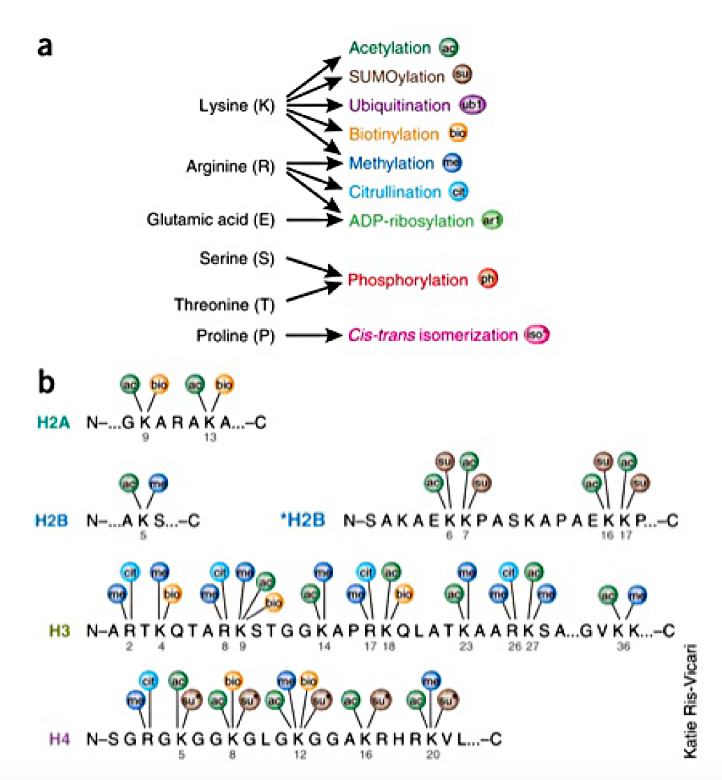
\includegraphics{images/figure1.png}
\caption{figure 1}
\end{figure}

    \textit{Figure 1: The histone modifications are named by the histone tail,
location in the protein sequence and the biochemical modification, e.g.
H3K4me3, refers to the trimethylation of the lysine (K) in the fourth
position in the protein sequence of histone 3 tail.}

    \begin{figure}[!h]
\centering
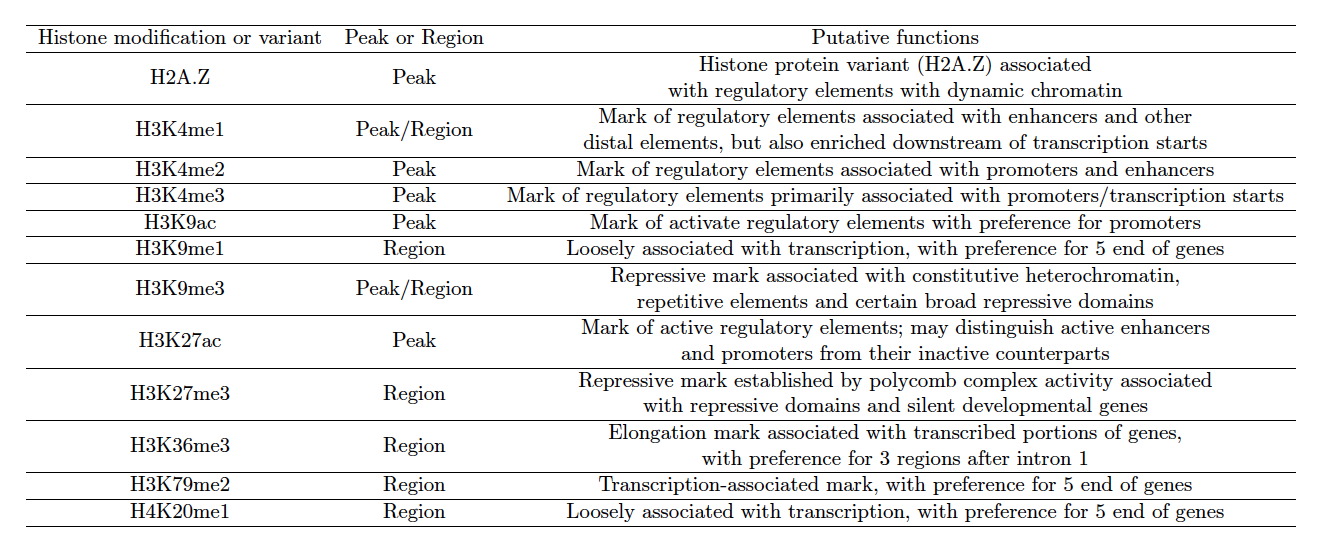
\includegraphics{images/figure2.png}
\caption{figure 2}
\end{figure}

    \textit{Figure 2: A summary of the putative functions of various histone
marks, according to the ENCODE Project.}

    \subsubsection{Transcription Start
Sites}\label{transcription-start-sites}

    It has been shown that the chromatin state, i.e. the combination of all
regulatory variations at the chromatin level, in the neighbourhood of a
gene has a large effect on its transcription. We will therefore start by
looking at the genome-wide profiles of the selected histone marks around
TSS.

    \textbf{Plot the distribution of H3K4me1 around protein-coding gene TSS
(this may take a few minutes to run).}

\begin{terminalinput}
\begin{Verbatim}[commandchars=\\\{\}]
\llap{\color{black}\LARGE\faKeyboardO\hspace{1em}} ngs.plot.r \PYZhy{}G hg19 \PYZhy{}O H3k4me1.tss \PYZhy{}FL \PY{l+m}{150} \PYZhy{}R cgi \PY{l+s+se}{\PYZbs{}}
        \PYZhy{}C H3k4me1.bam \PYZhy{}T H3k4me1
\end{Verbatim}
\end{terminalinput}

    \textbf{Q2: You can now view the H3K4me1 aggregation plots and heatmaps
in your folder. Where does the majority of the H3K4me1 signal appear in
relation to TSS?}

    \textbf{Q3: What proportion of genes display this pattern?}

    \textbf{Repeat these plots for other histone modifications.}

\begin{terminalinput}
\begin{Verbatim}[commandchars=\\\{\}]
\llap{\color{black}\LARGE\faKeyboardO\hspace{1em}} ngs.plot.r \PYZhy{}G hg19 \PYZhy{}O H3k4me3.tss \PYZhy{}FL \PY{l+m}{150} \PYZhy{}R tss \PY{l+s+se}{\PYZbs{}}
        \PYZhy{}C H3k4me3.bam \PYZhy{}T H3k4me3
\end{Verbatim}
\end{terminalinput}


    ngsplot also enables you to correct the ChIP sample using the control
sample. This aims to correct for any genome biases in alignability, GC
content etc.

    \textbf{Let's give this a try.}

\begin{terminalinput}
\begin{Verbatim}[commandchars=\\\{\}]
\llap{\color{black}\LARGE\faKeyboardO\hspace{1em}} ngs.plot.r \PYZhy{}G hg19 \PYZhy{}O H3k4me3\PYZus{}Control.tss \PYZhy{}FL \PY{l+m}{150} \PY{l+s+se}{\PYZbs{}}
        \PYZhy{}R tss \PYZhy{}C H3k4me3.bam:Control.bam \PYZhy{}T H3k4me3:Control
\end{Verbatim}
\end{terminalinput}


    \textit{Note: If you get an error about the alignment not being sorted,
try sorting your BAM file and using the sorted file instead.}

    You can now also plot the signal aroung specific annotated regions, such
as Ensembl gene bodies. H3K36me3 is known to be enriched over
transcribed genes.

    \textbf{Let's give this a try.}

\begin{terminalinput}
\begin{Verbatim}[commandchars=\\\{\}]
\llap{\color{black}\LARGE\faKeyboardO\hspace{1em}} ngs.plot.r \PYZhy{}G hg19 \PYZhy{}O H3k36me3 \PYZhy{}FL \PY{l+m}{150} \PYZhy{}R genebody \PY{l+s+se}{\PYZbs{}}
        \PYZhy{}C H3k36me3.bam \PYZhy{}T H3k36me3
\end{Verbatim}
\end{terminalinput}


    \textbf{Q4: Can you detect any patterns in this enrichment?}

    You can use configuration files in ngsplot to draw multiple graphs on
the same plot. For instance, we will plot multiple histone modifications
on the same plot, and also subset the genes, based on gene expression.

\newpage

Using a text editor, create the following tab-separated file, called
\texttt{multhist.txt} for drawing two histones modifications on the same
plot. -1 corresponds to looking at the whole genome.

    \begin{verbatim}
|-------------|----|---------|
| H3k4me1.bam | -1 | H3k4me1 |
| H3k4me3.bam | -1 | H3k4me3 |
\end{verbatim}

    \textbf{Run the following command to plot the graphs:}

\begin{terminalinput}
\begin{Verbatim}[commandchars=\\\{\}]
\llap{\color{black}\LARGE\faKeyboardO\hspace{1em}} ngs.plot.r \PYZhy{}G hg19 \PYZhy{}O H3k4me1.H3k4me3 \PYZhy{}FL \PY{l+m}{150} \PYZhy{}R tss \PY{l+s+se}{\PYZbs{}}
        \PYZhy{}C multhist.txt \PYZhy{}T H3k4me1.H3k4me3
\end{Verbatim}
\end{terminalinput}


    \textbf{Q5: Are the patterns you observe consistent with the putative
functions of the modification in the table given above?}

    \subsubsection{Gene Expression}\label{gene-expression}

    You will now use RNA-seq data form the same cell type results to
separate all of the Ensembl genes into three categories, based on the
expression (FPKM values) of the genes. The file containing the FPKMs for
GM12878 whole cell RNA-seq is called \texttt{genes.fpkm\_tracking}.
These FPKM values have been computed by Cufflinks.

    \textbf{Read the first few lines of the GM12878 whole cell
genes.fpkm\_tracking file.}

\begin{terminalinput}
\begin{Verbatim}[commandchars=\\\{\}]
\llap{\color{black}\LARGE\faKeyboardO\hspace{1em}} head \PYZhy{}n \PY{l+m}{10} genes.fpkm\PYZus{}tracking
\end{Verbatim}
\end{terminalinput}


    \textbf{Remove the header line.}

\begin{terminalinput}
\begin{Verbatim}[commandchars=\\\{\}]
\llap{\color{black}\LARGE\faKeyboardO\hspace{1em}} sed \PY{l+s+s1}{\PYZsq{}1d\PYZsq{}} genes.fpkm\PYZus{}tracking \PYZgt{} genes.fpkm.txt
\end{Verbatim}
\end{terminalinput}


    \textbf{Sort the genes by FPKM score.}

\begin{terminalinput}
\begin{Verbatim}[commandchars=\\\{\}]
\llap{\color{black}\LARGE\faKeyboardO\hspace{1em}} sort \PYZhy{}k10 \PYZhy{}n \PYZhy{}r genes.fpkm.txt \PYZgt{} genes.fpkm.sorted.txt
\end{Verbatim}
\end{terminalinput}


    \textbf{Count the number of genes.}

\begin{terminalinput}
\begin{Verbatim}[commandchars=\\\{\}]
\llap{\color{black}\LARGE\faKeyboardO\hspace{1em}} wc \PYZhy{}l genes.fpkm.sorted.txt
\end{Verbatim}
\end{terminalinput}


    \textbf{Use \texttt{head}, \texttt{sed} and \texttt{awk} to pull out the
Highest, Lowest and Intermediate expression genes.}

\begin{terminalinput}
\begin{Verbatim}[commandchars=\\\{\}]
\llap{\color{black}\LARGE\faKeyboardO\hspace{1em}} head \PYZhy{}n \PY{l+m}{5000} genes.fpkm.sorted.txt \PY{p}{|} \PY{l+s+se}{\PYZbs{}}
        awk \PY{l+s+s1}{\PYZsq{}\PYZob{}print \PYZdl{}1\PYZcb{}\PYZsq{}} \PYZgt{} high\PYZus{}expressed\PYZus{}genes.txt
\end{Verbatim}
\end{terminalinput}


\begin{terminalinput}
\begin{Verbatim}[commandchars=\\\{\}]
\llap{\color{black}\LARGE\faKeyboardO\hspace{1em}} awk \PY{l+s+s1}{\PYZsq{}\PYZob{} if(\PYZdl{}10 ==0) \PYZob{}print \PYZdl{}1\PYZcb{} \PYZcb{}\PYZsq{}} \PY{l+s+se}{\PYZbs{}}
        genes.fpkm.sorted.txt \PYZgt{} low\PYZus{}expressed\PYZus{}genes.txt
\end{Verbatim}
\end{terminalinput}


\begin{terminalinput}
\begin{Verbatim}[commandchars=\\\{\}]
\llap{\color{black}\LARGE\faKeyboardO\hspace{1em}} sed \PYZhy{}n \PY{l+s+s1}{\PYZsq{}10001,15000p\PYZsq{}} genes.fpkm.sorted.txt \PY{p}{|} \PY{l+s+se}{\PYZbs{}}
        awk \PY{l+s+s1}{\PYZsq{}\PYZob{}print \PYZdl{}1\PYZcb{}\PYZsq{}} \PYZgt{} mid\PYZus{}expressed\PYZus{}genes.txt
\end{Verbatim}
\end{terminalinput}


    \textbf{Create a tab-delimited configuration file expression.txt in a
text editor containing the following lines.}

    \begin{verbatim}
|--------------|--------------------------|--------|
| H3k27me3.bam | high_expressed_genes.txt | "High" |
| H3k27me3.bam | mid_expressed_genes.txt  | "Med"  |
| H3k27me3.bam | low_expressed_genes.txt  | "Low"  |
\end{verbatim}

    \textbf{Then run the following command.}

\begin{terminalinput}
\begin{Verbatim}[commandchars=\\\{\}]
\llap{\color{black}\LARGE\faKeyboardO\hspace{1em}} ngs.plot.r \PYZhy{}G hg19 \PYZhy{}R genebody \PYZhy{}C expression.txt \PY{l+s+se}{\PYZbs{}}
        \PYZhy{}O H3k27me3.express.genebody \PYZhy{}D ensembl \PY{l+s+se}{\PYZbs{}}
        \PYZhy{}FL \PY{l+m}{300} \PYZhy{}T H3k27me3.expression
\end{Verbatim}
\end{terminalinput}


    \textbf{Q6: What patterns can you see?}

    If you made it to here, well done!


    % Add a bibliography block to the postdoc



\end{document}
